\chapter{LArIAT: Liquid Argon In A Testbeam}\label{sec:experimentDescription}
\section{LArIAT \& the Intensity Frontier}
\section{The Particles Path to LArIAT}

LArIAT's home at Fermilab is the Fermilab Test Beam Facility (FTBF), where the experiment 
characterizes a beam of charge particles downstream from the Meson Center beam line. 

LArIAT's particles history begins in the Fermilab accelerator complex with a beam of protons. 
The process of protons acceleration develops in gradual stages, see picture \ref{fig:Accelerator}: gaseous hydrogen is ionized in order to form H$^{-}$ ions; these ions are boosted to 750 keV by a Cockroft-Walton accelerator and injected to the Linac linear accelerator that increases their energy up to 400 MeV; then, H$^{-}$ ions pass through a carbon foil and lose the two electrons; the resulting protons are then injected into a rapid cycling synchrotron, called Booster; at this stage protons reach 8 GeV of energy and are compacted into bunches; the next stage of acceleration is the Main Injector, a synchrotron which accelerates the bunches up to 120 GeV; in the Main Injector, several bunches are merged into one and used for the injection in the last stage.


The Fermilab accelerator complex works in supercycles of roughly 60 seconds in duration. The beam is then split by electrostatic septa and delivered at different experimental halls all over the lab. A 120~GeV$/c$ primary proton beam with variable intensity is extracted in four-second ``spills" and sent to the Meson Center beam line. Here, this primary beam is focused onto a tungsten target to create LArIAT's secondary beam. The composition of the secondary particle beam is mainly positive pions. For the LArIAT data considered in this work the secondary beam peak momentum was fixed at 64~GeV$/c$, although the beam is tunable in momentum between 8-80\,GeV$/c$; this was deemed a secondary beamline configuration which allowed a stable beam operation of the FTBF.
The beam of pions impinges then on a copper target within a steel collimator inside the LArIAT experimental hall (MC7) to create LArIAT tertiary beam, whose geometry in MC7 has been optimized for LArIAT (shown in  Fig.~\ref{fig:tert-layout}).   The steel collimator selects particles produced with a $13^\circ$ production angle at the target down the beamline.  The particles are then bend by  $~10^\circ$  through a pair of dipole magnets.  Tuning the magnets field intensity results in a range of particle momenta from 0.2 to 1.4~GeV/c.
The tertiary beam composition counts mostly pions and protons with a small fraction of electrons, muons, and kaons present as well. It is the job of the LArIAT beamline detectors to select the particles polarity,  to perform particle identification (beamPID) and to measure the momentum of the tertiary beam particles before they get to the LArTPC. The LArIAT detectors are described in the following paragraphs.  

%\begin{comment}     
\begin{figure}
  \centering  	
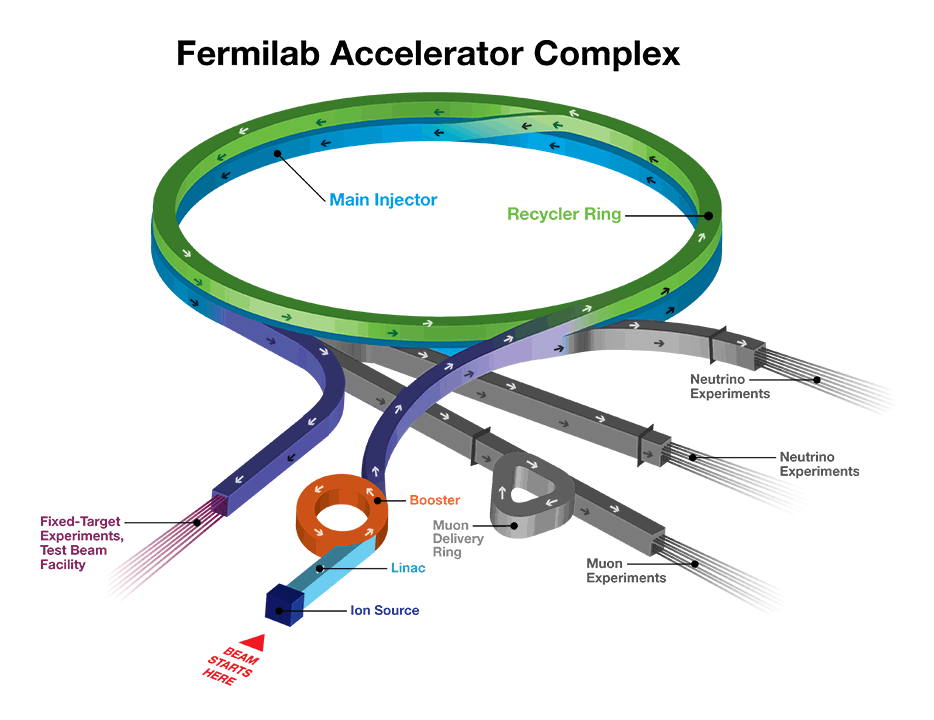
\includegraphics[width=\textwidth,height=\textheight,keepaspectratio]{Chapter-2/Images/AcceleratorFNAL.png}
\label{fig:Accelerator}
\caption{Layout of Fermilab Acellerator complex.}
\end{figure}

%\begin{comment}     
\begin{figure}
  \centering  	
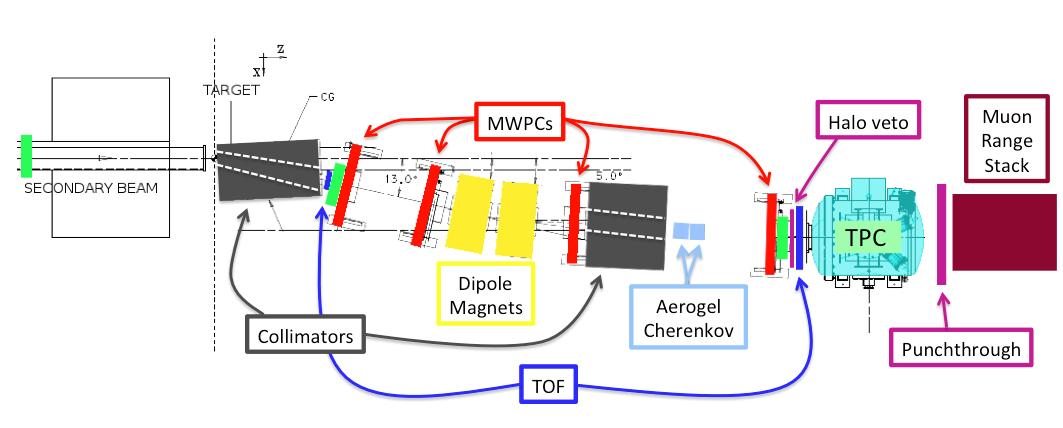
\includegraphics[width=\textwidth,height=\textheight,keepaspectratio]{Chapter-2/Images/Tertiary.png}
\label{fig:tert-layout}
\caption{Birds eye view of the LArIAT tertiary beamline. In grey: upstream and downstream collimators; in yellow: bending magnets in yellow; in red: wire chambers; in blue: time of flight; in green: liquid argon TPC volume; in maroon: muon range statck.}
\end{figure}


%%%%%%%%%%%%%%%%%%%%%%%%%%%%%%%%%%%%%%%%%%%%%%%%%%%%%%%%%%%%
\section{LArIAT Tertiary Beam Instrumentation}\label{sec:Instrumentation}

%%%%%%%%%%%%%%%%%%%%%%%%%%%%%%%%%%%%%%%%%%%%%%%%%%%%%%%%%%%%
The instrumentation of  LArIAT tertiary beam and the TPC components have changed several times during the three years of LArIAT data taking. The following paragraphs describe the components operational during the data taking period relevant to the hadron cross section measurements (a.k.a. Run II).

The components of the tertiary beamline instrumentation key for the hadron cross section analyses are the target and collimators system, the two bending magnets (in a similar configuration used for the  MINERvA T-977 test beam calibration~\cite{MinervaTestbeam}) a set of four wire chambers (WCs) and two time-of-flight scintillating paddles (TOF) and, of course, the LArTPC.  The magnets determine the polarity of the particles in the tertiary beam; the combination of magnets and wire chambers determine the particles momentum, which is used to determine the particle species in conjunction with the TOF.
A muon range stack downstream from the TPC and two sets of cosmic paddles configured as a telescope surrounding the TPC are also used for calibration purposes.


\subsection{Bending Magnets}\label{sec:Magnets}
%%%%%%%%%%%%%%%%%%%%%%%%%%%%%%%%%%%%%%%%%%%%%%%%%%%%%%%%%%%%
LArIAT uses a pair of identical Fermilab type ``NDB" electromagnets, recycled from the Tevatron's anti-proton ring \textcolor{red}{CITE CDF?}. 
The magnets are a fundamental piece of the LArIAT beamline as they are used in all the three tasks of the LArIAT beamline: the sign of the current in the magnet provide the selection of either positively or negatively charged particles, the value of the magnetic field is used in the momentum determination and the subsequent particle identification. 

We describe here the characteristics and response of one magnet. We expect the second one have a similar response, being identical in shape and with a similar history. The magnet aperture measures the gap dimensions to be 14.224~cm of height, 31.75~cm width, and  46.67~cm length.  The wire chambers aperture ($\sim$12.5~cm) is smaller than the magnet aperture, thus, only the central part of the magnet gap is utilized. The field is extremely uniform over this limited aperture and was measured with two Hall probes, both calibrated with nuclear magnetic resonance probes. The probes measured the excitation curve shown in Figure~\ref{fig:magnet_excitation}. 

\begin{figure}[!h]
\begin{centering}
\vspace{-0.3cm}
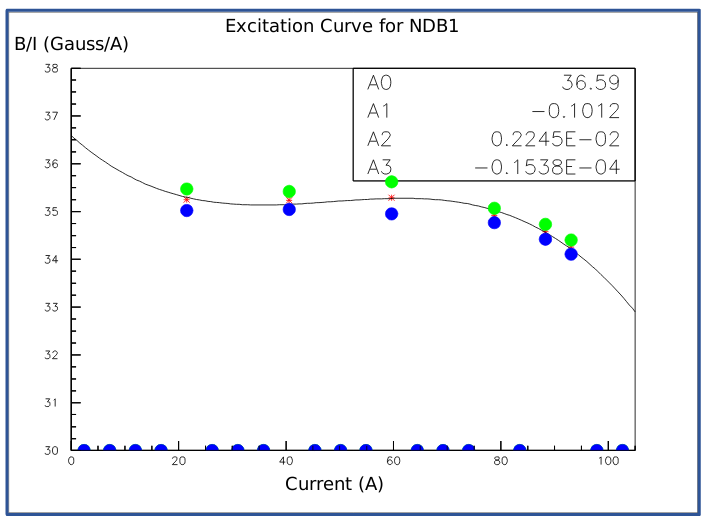
\includegraphics[height=3.0in]{Chapter-2/Images/ExcitationCurves.png}
\caption{
{ Magnetic field over current as a function of the current, for one NDB magnet (excitation curve). The data was collected using two Hall probes (blue and green). We fit the readings with a cubic function (black) to average of measurements (red) given in the legend.}
}
\label{fig:magnet_excitation}
\end{centering}
\end{figure}

The current being passed through the magnets at a given time is identical in both magnets. For Run II period, the current settings explored were 60A (B $\sim$0.21 T) and 100A (B $\sim$0.35 T) in both polarities. 
Albeit advantageous to enrich the tertiary beam composition with high mass particles such as kaons, we never pushed the magnets current over 100 A, not to incur in overheating.  During operation, we operated a air and water cooling system on the magnets and we remotely monitored the magnets temperature.
 
\subsection{Multi-Wire Proportional Chambers}\label{sec:MWPC}
%%%%%%%%%%%%%%%%%%%%%%%%%%%%%%%%%%%%%%%%%%%%%%%%%%%%%%%%%%%%
\begin{figure}[!h]
\begin{centering}
\vspace{-0.3cm}
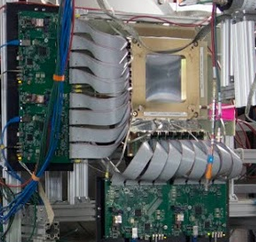
\includegraphics[height=2.3in]{Chapter-2/Images/WireChamber.png}
\caption{
{One of the four Multi Wire Proportional Chambers (WC) used in the LArIAT tertiary beamline.}
}
\label{fig:wirechamber}
\end{centering}
\end{figure}

LArIAT uses four Multi-Wire proportional chambers, or wire chambers (WC) for short, two upstream and two downstream from the bending magnets. The geometry of one chamber is shown in Figure~\ref{fig:wirechamber}: the WC effective aperture is a square of  12.8~cm perpendicular to the beam direction.  Inside the chamber, the 128 horizontal and 128 vertical wires hang at a distance of 1~mm from each other in a mixture of 85\% Argon and 15\% isobutane gas.  The WC operating voltage is between 2400 V and 2500 V. LArIAT wire chambers are an upgraded version of the Fenker Chambers~\cite{Fenker}, where an extra grounding improves the signal to noise ratio of the electronic readout.  

Two ASDQ chips~\cite{ASDQchip} mounted on a mother board plugged into the chamber serve as front end amplifier/discriminator. The chips are connected to a multi-hit TDC~\cite{Sten} which provides a fast OR output used as first level trigger. The TDC time resolution is 1.18~ns/bin and can accept 2 edges per 9~ns.  
The maximum event rate acceptable by the chamber system is of 1 MHz: this rate is not a limiting factor considering that the rate of the tertiary particle beam at the first wire chamber is estimated to be less than 15 kHz. A full spill of data occurring once per supercycle is stored on the TDC board memory at once and read out by a controller specially designed controller.  We use LVDS cables to carry both power and data between the controller and the TDCs and from the controller to the rest of the DAQ.  
%It is possible to program the time window for acceptance for hits, time offsets, front end threshold, and pulse shaping parameters through the controller via a USB from a PC or through an Ethernet connection.

\subsubsection{Multi-Wire Proportional Chambers functionality}\label{sec:MWPCfunc}


\subsection{Time-of-Flight System}\label{sec:TOF}
%%%%%%%%%%%%%%%%%%%%%%%%%%%%%%%%%%%%%%%%%%%%%%%%%%%%%%%%%%%%
Two scintillator paddles, one upstream to the first set of WCs and one downstream to the second set of WCs  form LArIAT  time-of-flight (TOF) detector system. 

 \textcolor{red}{find exact dimentsions}
The upstream paddle is made of a 10 x 6 x \textcolor{red}{?}~cm scintillator piece, read out by two \textcolor{red}{Hamamatsu 2 inch} PMTs mounted on the beam left side which collect the light from light guides mounted on all four edges of the scintillator. The downstream paddle dimensions are  14 x 14 x \textcolor{red}{?}~cm and it is read out by two \textcolor{red}{Hamamatsu 2 inch} PMTs on the opposite ends of the scintillator.
The relatively thin width on the beamline direction minimizes energy loss of the particles coming from the target in the scintillatior material.

\begin{figure}[!h]
\begin{centering}
\vspace{-0.3cm}
%\includegraphics[height=2.3in]{figures/tofdelay.png}
\caption{
{\scriptsize \sf Pictures of the TOF system as was deployed during Run-I and Run-II data taking. The left image is of the upstream TOF paddle and the right image is of the downstream TOF paddle }
}
\label{fig:TOFSystemRunIandII}
\end{centering}
\end{figure}



The CAEN 1751 digitizer is used to digitize the TOF PMTs signals at a sampling rate of 1 GHz. The 12 bit samples are stored in a circular memory buffer. At trigger time, data from the TOF PMTs are recorded to output in a 28.7 $\mu$ second windows starting  approximately 8.4 $\mu$sec before the trigger time. 



\subsubsection{TOF functionality}\label{sec:MWPCfunc}


The TOF signals rise time (10-90\%) is 4 ns and a full width, half-maximum of 9 ns consistent in time. The signal amplitudes from the upstream TOF and  downstream TOF are slightly different:  200 mV for the upstream PMTs but only 50 mV for downstream PMTs. 

The time of the pulses was calculated utilizing an oversampled template derived from the data itself. The pulse pedestal was taken from samples far from the pulse and subtracted to the pulse amplitude. We then stretch vertically a template to match the pedestal-subtracted pulse amplitude and we move it horizontally to find the time. With this technique, we find a pulse time-pickoff resolution better than 100 ps.  The pulse pile up is not a significant problem given the TOF timing resolution and the rate of the particle beam.  Leveraging on the pulses width uniformity of any given PMT (sigma of 400 ps),  we flag events where two pulses overlap as closely in time as 4 ns with an 90\% efficiency according to simulation. 


We combine the pulses from the two PMTs on each paddle to determine the particles' arrival time by averaging the time measured from the single PMT, so to minimize errors due to optical path differences in the scintillator.  However, a time spread of approximately 300~ps is present in both the upstream and downstream detectors, likely due to transit time jitter in the PMTs themselves.  There is no evidence of systematic timing drift over long periods such as 3-4 months of a data-taking: the maximum variation of the average time differences between pairs of PMTs reading out the same scintillator is of the order of 150~ps.



\section{In the Cryostat}

\subsection{TPC: Charge Collection}\label{sec:TPC}
\subsection{TPC: Light Collection System}
\subsection{Cryogenics and Purity Control}
\subsection{TPC: Electric Field Measurement}
\section{Trigger and DAQ}
\section{Control Systems}

\begin{comment}




%%%%%%%%%%%%%%%%%%%%%%%%%%%%%%%%%%%%%%%%%%%%%%%%%%%%%%%%%%%%
\subsubsection{Punch-Through and Muon Range Stack Instruments}\label{sec:MuRS}
%%%%%%%%%%%%%%%%%%%%%%%%%%%%%%%%%%%%%%%%%%%%%%%%%%%%%%%%%%%%


%%%%%%%%%%%%%%%%%%%%%%%%%%%%%%%%%%%%%%%%%%%%%%%%%%%%%%%%%%%%
\subsection{LArIAT Cosmic Ray Paddle Detectors}\label{sec:CosmicRayPaddle}
%%%%%%%%%%%%%%%%%%%%%%%%%%%%%%%%%%%%%%%%%%%%%%%%%%%%%%%%%%%%

LArIAT's system to trigger on cosmic rays is based on two so-called "cosmic towers" which stand  upstream and downstream of the cryostat, one on beam's right and one on beam's left, framing the cryostat.  Each cosmic tower is composed of two paddle assemblies, upper and lower.  The paddle assemblies each consist of four paddles, a matched pair which stand upright and a second matched pair lying across the top  of the assembly, to act as a veto for downward-going cosmic ray air showers.  Unless vetoes by the horizontal paddles, signals from paddle assemblies along the body diagonals of the TPC are combined in a logical ``AND'' to select cosmic muons crossing the TPC along one of its diagonals. A high proportion of events triggered this way contain cosmic ray tracks crossing both anode and cathode.  Such tracks provide a sample of LAr ionization with effectively uniform linear ionization density, but experience the entire range of charge attenuation available in the TPC before they drift to the anode. These tracks are used to calculate and monitor the level of electronegative contaminants in the liquid argon and provide a calibration sample for calorimetry and electric field studies outlined in Section \ref{sec:DetectorPerformance}.

The paddles have trapezoidal shape and are each enclosed in an aluminum case. An example is shown in Fig. \ref{pic:cosmicpaddle}. They come in two different sizes: a smaller version, with bases $32.2~cm$ and $26.7~cm$, $61.0~cm$ height and $3.02~cm$ thickness, and a bigger version, with bases $33.2~cm$ and $27.0~cm$, $70.8~cm$ height and $3.02~cm$ thickness. Each paddle is equipped with wavelength-shifting optical fibers running along one of the long sides and optically coupled to a low voltage, Zener-diode Hamamatsu H5783 PMT.  Signals from the PMT are amplified and discriminated by a custom-made PMT Amplifier and Discrimination (PAD) circuit mounted at one end of the paddle, then sent through a CAT5 cable to a Control and Concentrator Unit (CCU) which both power the PMT, controlling voltage and threshold, and output the PMT signal as logic ECL pulse.

\begin{figure}[h!]
 \centering
% 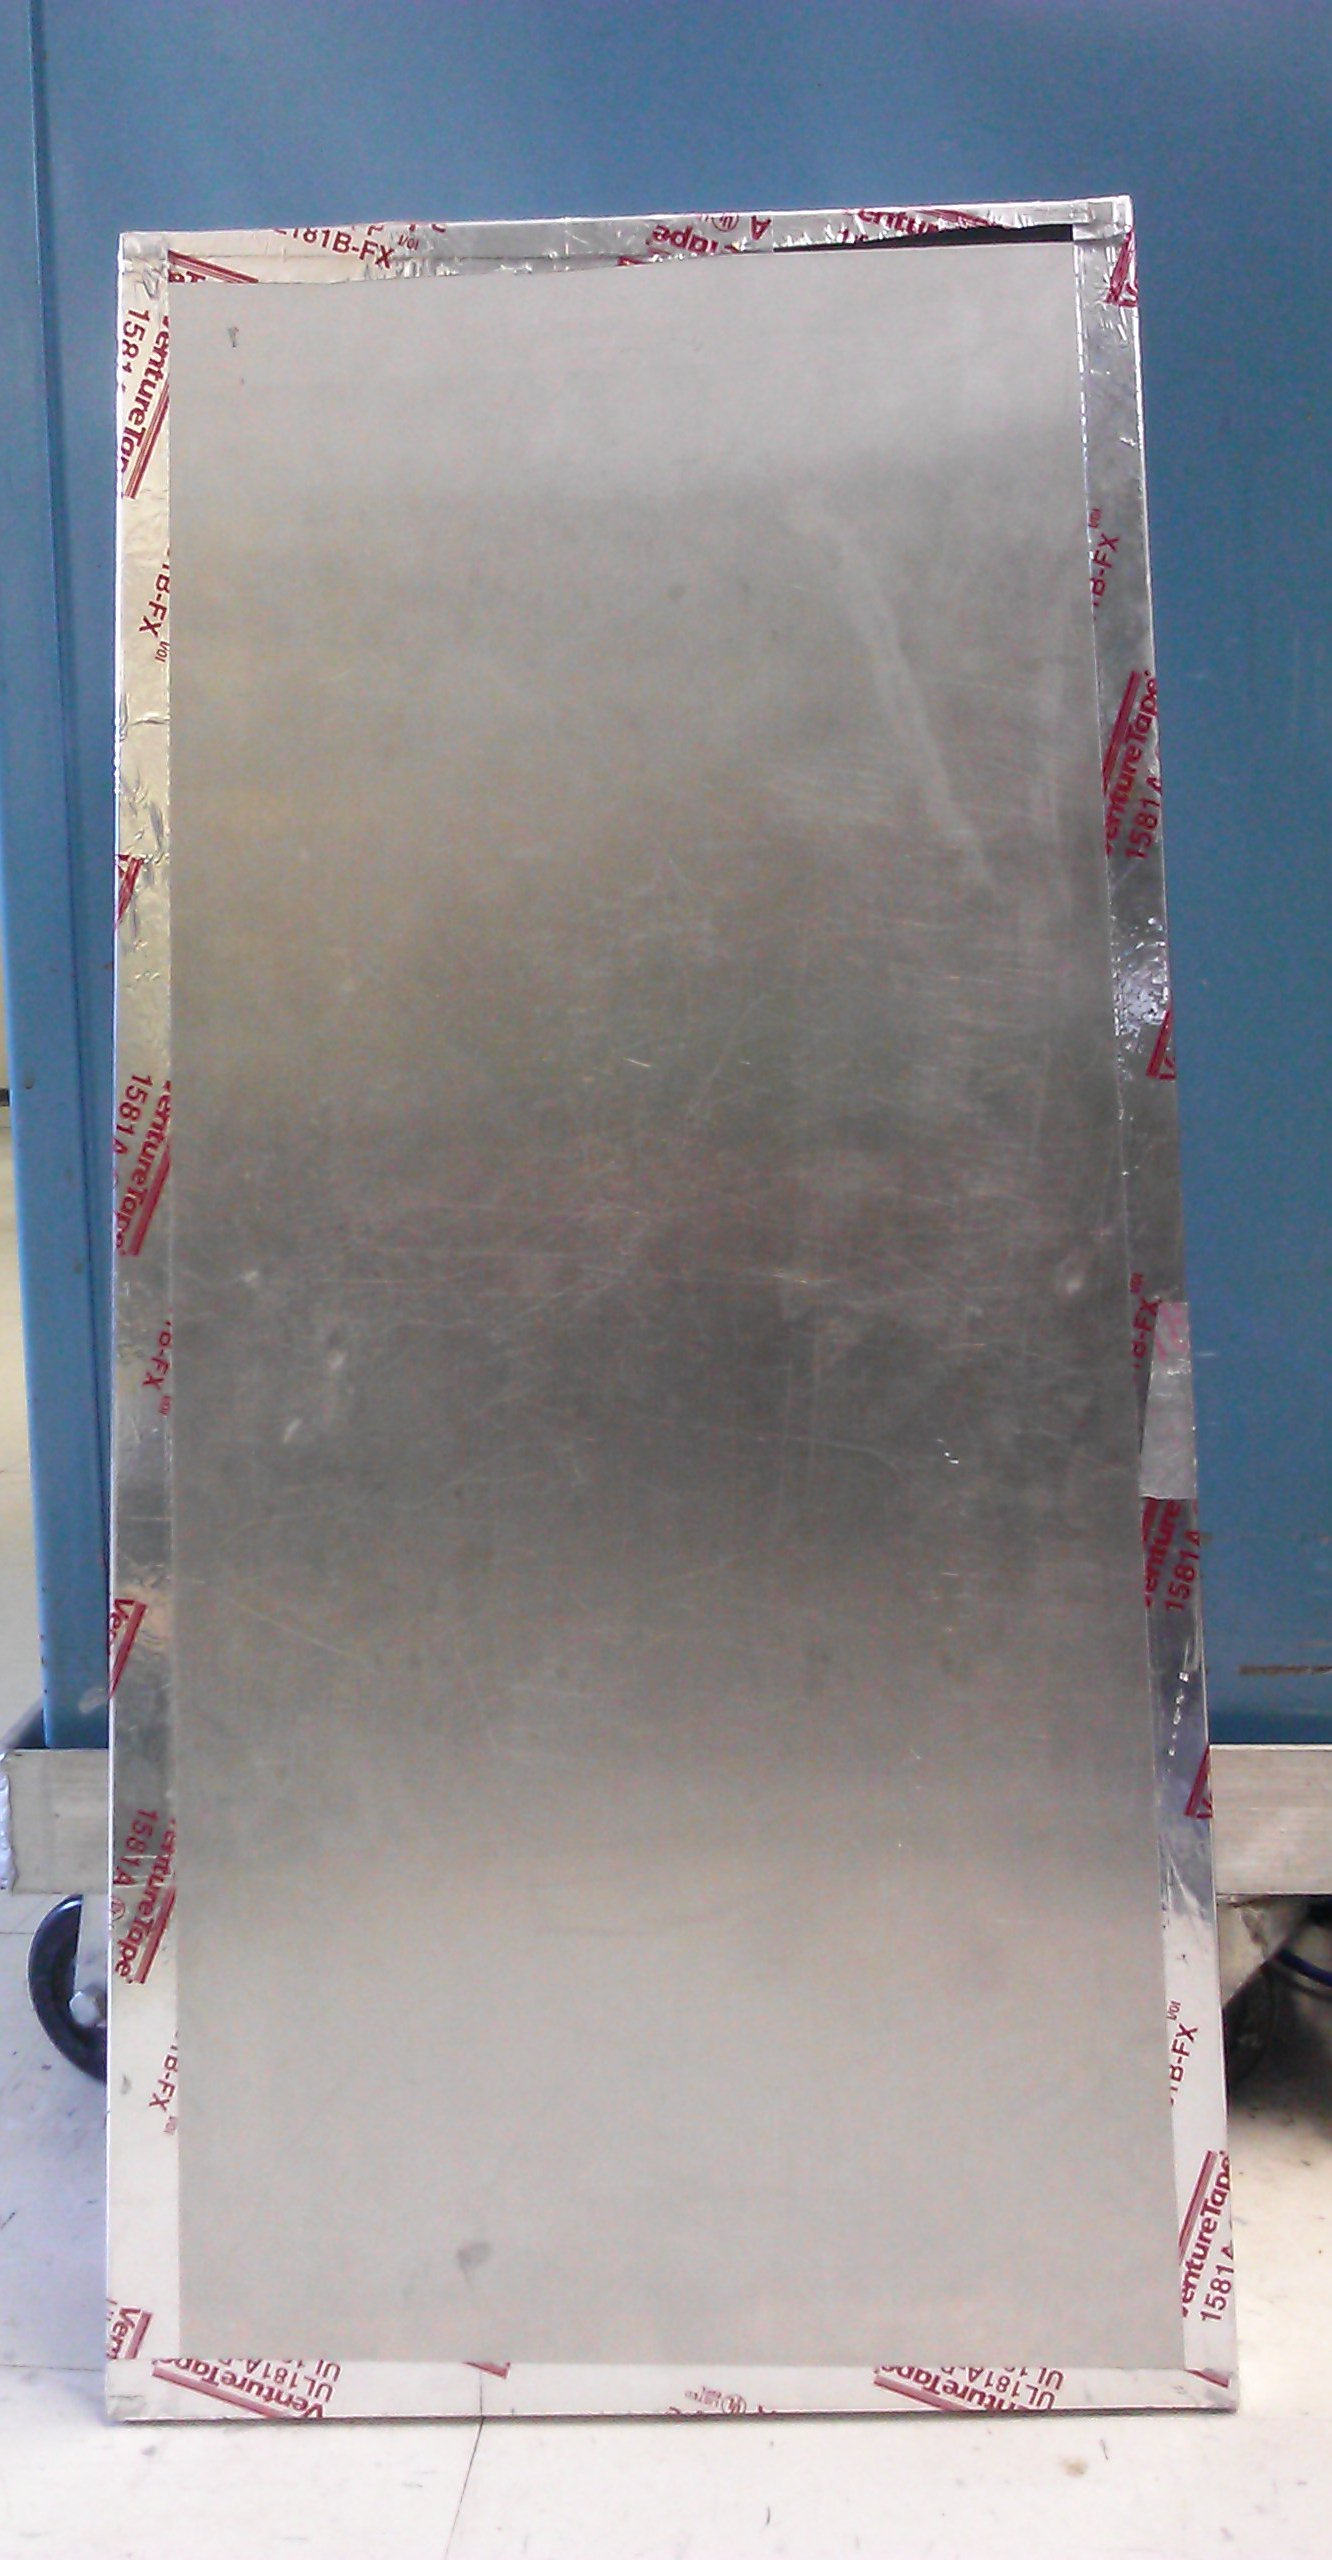
\includegraphics[angle=90,width=0.7\textwidth]{figures/Cosmic_Paddle.jpg}
\caption{
Photograph of one of the scintillation counters used in the cosmic towers. 
} 
\label{pic:cosmicpaddle}
\end{figure}

The paddles were selected from a pool of over 300 scintillating counters collected during the decommissioning of the CDF detector at Fermilab. 
For each counter, both the efficiency $\varepsilon_P$ and the noise $\eta_P$ as a function of the voltage were determined. The measurement was performed sandwiching the given paddle among 4 sample counters, placed two above and two below the paddle under test. The efficiency 
$\varepsilon_P$ was defined as the ratio between the 5-fold coincidence and the 4-fold coincidence of the sample counters. The accidental rate $\eta_P$ was instead defined as the number of 5-fold coincidence observed during ten minutes of data acquisition, when the signal of the paddle under test was delayed by $5 \mu s$. Each paddle with $\varepsilon_P \geq 95\%$ and $\eta_P = 0$ at working voltage was identified as a candidate for the Cosmic Ray system. The ones with the highest efficiency and lowest single count rate were then selected to realize the system itself. 
The plot of $\varepsilon_P$ as a function of the PMT voltage for one example paddle is shown in Fig. \ref{pic:CR_Effplot}.

\begin{figure}[h!]
 \centering
% \includegraphics[width=0.7\textwidth]{figures/TSU29_Efficiency.png}
\caption{
Plot of the counter efficiency $\varepsilon_P$ as a function of the PMT voltage for one of the paddles composing the Cosmic Ray system. 
} 
\label{pic:CR_Effplot}
\end{figure}


%$\varepsilon_P$ at a given voltage is defined as:

%$$
%\varepsilon_P = \frac{R_{1-2} \land R_{3-4} \land R_P}{R_{1-2} \land R_{3-4}}
%$$

%where $R_P$ is the rate of the paddle $P$ to be tested, $R_{1-2}$ is the coincidence rate of two sample paddles positioned above $P$, while $R_{3-4}$ is the coincidence rate of two sample paddles positioned below $P$.
%$\eta_P$ at a given voltage is instead defined as:

%$$
%\eta_P = \frac{R_{1-2} \land R_{3-4} \land R_{P^*}}{R_{1-2} \land R_{3-4}}
%$$

%where $R_{P^*}$ is the Rate of the paddle $P$ 


The trigger rate $R$ of the whole system is $R=0.032Hz$, corresponding to $\sim 1.9~\mu/minute$.
\end{comment}

